\documentclass{article}
\usepackage[margin=1in]{geometry}
\usepackage{url}
\usepackage{graphicx}
\graphicspath{ {./images/} }

\pagenumbering{arabic}

\title{Installing XPDP1: Linux Edition}
\author{}
\date{Last updated: August 2018}

\begin{document}
	\maketitle
	
	\noindent \textbf{NOTE 1}: This tutorial is based on the desktop/workstation edition of Ubuntu 16.04.3 LTS and 18.04 64 bit and should also work for Windows Subsystem for Linux. \\
	\textbf{NOTE 2}: For further information on the XPD family of codes (as well as previous editions), please see \url{http://ptsg.egr.msu.edu/} \\
	
	\noindent XPDP1 is the planar 1D Particle-in-Cell (PIC) code developed by The Plasma Theory and Simulation Group (PTSG) formerly at the University of California at Berkeley and now at Michigan State University. This guide is a walkthrough of how to install XPDP1 (and its dependency XGRAFIX) on Ubuntu Linux, taking into account a few changes we need to make to run on newer Linux distros (since the code editions we're using are several years old). It is assumed that the reader is proficient in navigating the Ubuntu Terminal, installing programs via command line, editing plaintext files (in an editor like \verb|gedit|), etc.
	
	\section{Installing XGRAFIX}
	
	\noindent XGRAFIX is the display tool used for XPDP1, and it needs to be be installed first.
	\begin{enumerate}
		\item Download the tar.gz archive file for XGRAFIX from \\ \url{http://ptsg.egr.msu.edu/pub/codes/xgrafix.tar.gz} using \verb|wget "http://..."|
		
		\item Using Archive Manager, extract the tar file to the directory where you'd like to store the XGRAFIX files (\verb|~/Documents/| or another location -- i.e. NOT your Downloads folder -- is recommended!) using \verb|tar -xvf xgrafix.tar.gz|
		
		\item Before we get started installing XGRAFIX directly, some dependencies are needed. Open a Terminal window, and type:
		\begin{verbatim}
			        sudo apt-get install gcc g++ build-essential automake 
			             tk8.6-dev imagemagick bison libx11-dev libxpm-dev
			             fftw-dev libfftw3-dev h5utils hdf5-tools libhdf5-dev
		\end{verbatim}
		
		typing in your administrator password when prompted.
		\begin{enumerate}
			\item[NOTE:] We're using Tcl/Tk version 8.6 here, which is the newest edition. The editions of XGRAFIX (2.70.2) and XPDP1 (4.11) that we're using are compatible with both versions 8.5 and 8.6. If you require Tcl/Tk 8.5 in some other code/program, don't worry; multiple versions can be installed on the same machine!
		\end{enumerate}
		
		\item Now we need to modify the configuration script to better fit our system. In the \verb|xgrafix| folder that you extracted, look for the file \verb|run_conf.sh| and open it in a plaintext editor. 
		\begin{enumerate} 
			\item[NOTE:] You have several options here, including changing the preferred install location, enabling MPI (I would not recommend this as the newest version of OpenMPI is not compatible with XGRAFIX. Changing XGRAFIX to fit would be rather time-consuming!), and adding configuration options, using the \verb|confopts| variable near the top of the file. 
		\end{enumerate}
		
		\item Make sure that the variable \verb|precision=double| (not \verb|float|). It will cause an error later on if it is set to \verb|float|. Change \verb|confopts| to the following:
		\begin{verbatim}
			        
			        libdir="/usr/lib/x86_64-linux-gnu/"
			        incdir="/usr/include/"
			        tcltkver="8.6"
			        confopts="--prefix=$prefix --with-SCALAR=$precision --enable-fulloptimize
			                  --with-XGRAFIX-lib=$prefix/lib --with-XGRAFIX-include=$prefix/include
			                  --with-tclconfig=${libdir}/tcl${tcltkver} --with-tkconfig=${libdir}/tk${tcltkver}
			                  --with-tclhdir=${incdir}/tcl${tcltkver}"
		\end{verbatim}
		
		
		\item We may need to tell the configuration script where to find library directories for the Tcl/Tk programs required for the installation. Find the line \verb|echo "configuring with options: $confopts"| and add the following two lines immediately below it (above \verb|./configure $confopts && \|):
		\begin{verbatim}
		            TCL_LIBDIR_PATH=/usr/lib/x86_64-linux-gnu/ \
		            TK_LIBDIR_PATH=/usr/lib/x86_64-linux-gnu/ \
		\end{verbatim}
		
		\item We're now ready to run the configure script! Save \verb|run_conf.sh|, and open your Terminal. Changing to the \verb|xgrafix| directory, run the command \verb|sh run_conf.sh| and wait for the script to finish. If successful, you should see the following message: 
		\begin{verbatim}
		        Configure successful!
		         if you have a multicore machine, now you can build with:
		         'make -j 4' (for 4 threaded compiling)
		         and install with:
		         'make install' or 'sudo make install', depending on whether you have write
		         permissions to /usr/local/"
		\end{verbatim}
		
		\item Now, enter the command \verb|make -j 4| in order to build the XGRAFIX program for your machine. Note that you may need to enter \verb|sudo make -j 4| if you are using Ubuntu on Windows. This can continue for a couple minutes. When it finishes, enter the command \verb|sudo make install| to install XGRAFIX onto your system. 
		
		\item To make sure everything is working correctly, we need to test our XGRAFIX installation. In the terminal, navigate to the \verb|ctest| directory inside of the \verb|xgrafix| directory we've been working in so far. Type \verb|xtest|. You should see several windows pop up - a 3D Surface Plot, a list of sample diagnostic plots, and a control panel. Test a couple plots by opening them, and if they open without issue, close XGRAFIX by selecting Quit on the Control Panel. 
	\end{enumerate}
	\noindent If the test was successful, XGRAFIX is successfully installed! If you would like to see the original installation instruction packaged with XGRAFIX, please refer to the README file located in the \verb|xgrafix| directory.
	
	\section{Installing XPDP1}
	
	\begin{enumerate}
		\item Download the tar.gz archive file for XPDP1 from \url{http://ptsg.egr.msu.edu/pub/codes/xpdp1.tar.gz}
		
		\item Using Archive Manager, extract the tar file to a directory where you'd like to store the XPDP1 files. The same location where you extracted the XGRAFIX files is recommended!
		
		\item Open the \verb|xpdp1| directory, and then navigate to the \verb|src| directory.
		
		\item Using your favorite plaintext editor, open the file \verb|makefile|. 
		
		\item Make sure that the \verb|XGRAFXPATH| variable near the top of the file is set to the correct install location of XGRAFIX.
		
		\item Save \verb|makefile|, and close the text editor.
		
		\item Open a Terminal window, and navigate to the \verb|src| directory. Enter the command \verb|make -j 4| to build XPDP1, just like we did with XGRAFIX. If it is successful, the build should finish and return you to a command prompt. 
		
		\item We now need to test XPDP1 using one of the sample files located in the \verb|inp| directory. Return to the \verb|xpdp1| directory in your Terminal, and run the command \verb|./xpdp1 -i ./inp/ambipolar.inp|. You should see the Diagnostics and Control Panel windows of XGRAFIX open.
		
		\item The diagnostics listed should be various plasma parameters and values. Find and select \verb|N(x)| and press Open to see a plot of density with respect to spatial dimension \textit{x}. Press Run in the Control Panel Window to begin the simulation. If the simulation proceeds, you should see something like Figure 1 in the plotting window. 
		
		\begin{figure}[h!]
			\caption{Sample XPDP1 Output for N(x).}
			\centering
			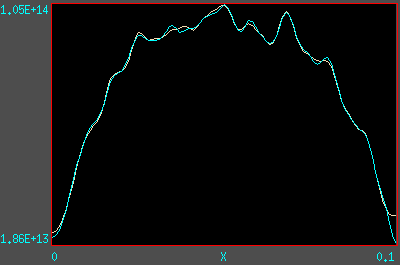
\includegraphics[width=0.5\textwidth]{ambipolar.png}
		\end{figure}
		
		\item To enable running XPDP1 when inside any directory, it needs to be added to our system PATH. In order to this, open up your \verb|.bashrc| file located in your home directory inside of a plaintext editor. At the bottom of the file, add the following at the end of the file: 
		\begin{verbatim}
		        export PATH="/home/$USER/Documents/PTSG/xpdp1/:$PATH"
		\end{verbatim}
		Change \verb|/home/$USER/Documents/PTSG/xpdp1/| to the directory path of the location where you installed XPDP1.
		
		\item Save \verb|.bashrc| and restart your machine (or enter: \verb|. ~/.bashrc|).
	\end{enumerate}
	
	\noindent XPDP1 is now installed and configured! To read the full XPDP1 documentation, see the file \verb|xpdp1_manual.ps| file inside of the \verb|doc| directory, which can be opened natively in Ubuntu. To create this file in another format (like PDF) run the \verb|xpdp1_manual.tex| file in a compatible PDF\LaTeX \hspace{1pt} compiler. To see a quick rundown of how to use the XPDP1 command at any time, simply type \verb|xpdp1 --help| in any Terminal command prompt. 
\end{document}